\begin{problem} (20 points)
  
  \noindent
  Create a Crow’s Foot ERD to include the following business rules for the ProdCo company:
    \begin{itemize}
      \item Each sales representative writes many invoices.
      \item Each invoice is written by one sales representative.
      \item Each sales representative is assigned to one department.
      \item Each department has at least one sales representative.
      \item Each customer can generate many invoices.
      \item When a new customer is added that customer may or may not have any invoices.
      \item Each invoice is generated by one customer.
    \end{itemize}
\end{problem}
\begin{Answer}
  In MySQL Workbench, I couldn't find an option
  to specify ``one-to-many'' without specifying the lower
  limit of either $0$ or $1$.
  So I deduced what further constraints might hold:
  
  \begin{itemize}
    \item New sales representatives might not have an invoice yet, so
    I made that relationship \crim{zero-or-many} on the side of the invoice.
    \item I deduced that each invoice must have a customer, so I made
    that relationship \crim{one-and-only-one} on the side of the customer.
  \end{itemize}
  \bigskip
  \centering
  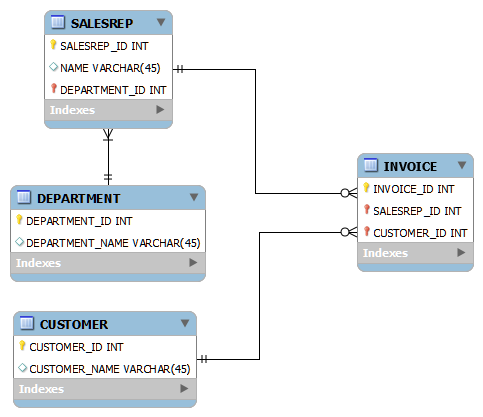
\includegraphics[scale=0.8]{erd.png}
\end{Answer}
